\chapter{Introduction}
Distributed sensor networks (DSNs) consist of any number of sensors that collect and sense information about the physical environment around them. The sensors that make up these networks can either be homogeneous or heterogeneous. Distributed sensor networks are dynamic in that sensors can be added or removed from the network at any time. DSNs also increasingly include mobile sensors as well. With the onset of the Internet of Things (IoT), its easier than ever to build and deploy distributed sensor networks. Further, mobile devices, such as mobile phones, are seeing increased usage as intelligent sensing agents.

Distributed sensor network (DSN) optimization is a broad topic with many different facets to consider. Much of the literature on the topic focuses on optimizing data flow between sensors as data flows from sensor to sensor and eventually to a sink. 

The focus of this dissertation however, is to deal with the challenges of a specific subset of DSNs. That subset is DSNs where data always flows directly from each sensor in the network to sink nodes, thus, eliminating the need to worry about intra-sensor communication, networking, and routing. 

There are a broad range of technical challenges beyond the data sink. The introduction of the Internet of Things (IoT) has created an explosion of internet connected devices that sense a massive number of attributes about the physical world surrounding them. An increase in sensors has created an increase in multimodal data generation with the inverse problem of creating a decrease in the signal-to-noise ratio, making it more difficult to identify and classify signals of interest. Multimodal data provides challenges for analysis algorithms because each sensor may be streaming multiple physical features that need to be analyzed and dealt with independently and dependently. As the densities of sensors increase, analysis must be able to work with missing data, incorrect data, incomplete data, and data coming from a heterogeneous mix of hardware and sensor configurations. Further, we can no longer assume that sensors are static in time and location as mobile sensors are quickly becoming more prevalent, making analysis trickier. All of these issues require an increase in storage and computational resources. Therefore, we must find approaches to deal with sensor data to lessen these hurdles.

As DSNs scale, available storage must be balanced with the amount of data being retained. Further, once data is collected, we need strategies for turning sensor data into actionable data and insights. This generally involves detecting and classifying signals of interest. It's these last two important DSN challenges that are the focus of this dissertation.

\section{Converting Sensor Data into Actionable Insights}
Data collected from sensors is often a sampled payload of data points representing some feature in the physical world. As examples, weather stations produce sampled features relating to temperature, wind speed, and humidity, power meters produce a metric of total electricity consumed, power quality sensors produce sampled data points which include voltage, frequency, and THD, and infrasound networks produce sampled data which represent audio waveforms.

These features by themselves, while interesting, do not provide any context as to if there is a signal, what the signal is, when and where the signal came from, or what caused the signal in the first place. Detection and classification algorithms are used to attempt to extract some of these properties. Primitive data is aggregated and compared to other primitive data to find correlations in both time and space. Data is compared to historic data in an attempt to find patterns or other similarities. This type of data is more interesting in that we might learn more about a signal using these techniques, but they still don't provide actionable insights or causality information. Further, the problem of providing actionable insights is highly dependent on the sensing domain. Depending on other available sources of data, providing data fusion and context from outside of the DSN can be difficult.

\section{Big Data Management in DSNs}
Big Data is generally defined by the four V's; volume, velocity, variety, and value. These characteristics can be observed in many of the DSNs that exist and are being created today.

That is, distributed sensor networks create a large volume of data due to the abundance of IoT and mobile devices that make up DSNs. As communication infrastructures improve and hardware becomes smaller, smarter and more energy efficient, sensors are able to send and transfer larger amounts of data. The ease of building and deploying sensors in DSNs means that more sensors can be produced much more cheaply allowing for more sensors to be used within a DSN, increasing coverage, but also increasing the volume of data.

Distributed sensor networks create a variety of data with different formats and data quality issues. Distributed sensor networks can produce data at high velocity. These characteristics of data produced from distributed sensor networks create a need for efficient architectures and specific algorithms designed for working with Big Data.

Further, sensor networks are often constrained in both computing power and available energy sources. This forces us to find comprises between data collection, onboard sensor processing, sensor communication, and network coordination.

As DSNs scale, the amount of data a DSN must store and process increases. At certain scales, DSNs simply can not store and process all of the primitive data that sensors are producing or process and store aggregate data products that detection and analysis routines produce. Designers of a DSN can either choose to collect and keep all data forever (from raw data to generated products), or they can implement strategies for systematically discarding (hopefully) non-interesting data. If the first option is chosen, then there is no risk of accidentally discarding signals of interest and data can be reanalyzed when analysis algorithms change or are tweaked. However, storage and analysis of such amounts of data can cause system degradation or even be unfeasible. If the second option is chosen, processes must be put in place that attempt to only store ``interesting" data and discard sensor noise.  The second option runs the risk of discarding important data and old data can not be reanalyzed under this approach. However, this approach provides the benefits of providing predictable data storage requirements that can be tuned and optimized for a particular domain and DSN.

%\subsection{DSN Data Collection Schemes}
%Data can be collected from DSNs in various ways. Sensors can store data onboard to be collected manually or transmit data via a multitude of mediums (satellites, radio, laser, wired connections) using a slew of standards (TCP/IP, Zigbee, Bluetooth, custom, etc).
%
%In some DSNs, data is routed between the sensors using various approaches and eventually makes its way to a sink or sinks. A sink is a data collection node. Cloud computing has become a prevalent choice for DSN sinks since they often provide the ability to provision resources as needed. Various approaches have been proposed that minimize and optimize communications between sensors within a DSN.
%
%In other DSNs, sensor nodes have direct access to a sink, and instead of communicating with each other and passing messages among themselves, the nodes send their data directly to the sink. It's also possible for a DSN to take a hybrid approach and performs some communication within the network and some directly to the sink.
%
%Not only are there various approaches to routing data, but there are also various approaches to deciding what kind of data to send (or acquire).
%
%\subsection{DSN Detection Schemes}
%On one extreme end, we have the send everything approach where each sensor sends its data to the sink all the time (or at least when it has the means to do). In this scenario, the sink is responsible for collection, cleaning, detection, and classification of signals and events within the data. This approach can be bandwidth and energy intensive, but provides the benefit of allowing more complete analysis to occur beyond the sink where more computational resources exist. This provides more accurate results and allows the sink to examine the results in aggregate with the rest of the DSN.
%
%The other extreme is that sensors only send data when they have detected a signal of interest. In this scenario, sensors use onboard computing capabilities to filter their sensor stream and perform signal detection on the device. Only when the devices make a detection do they send the detection or data stream to a sink for further processing. This minimizes bandwidth but detection and classification of signals must occur with more constrained computing and energy environments. Further, the global state of the network can't be known without adding the complexity of sensor-to-sensor communication.
%
%Often time a hybrid approach is taken where low fidelity feature extracted and sometimes aggregate data is sent from the sensors to the sink. The sink analyzes the low fidelity feature extracted stream to determine if raw data should be requested from the sensors. The act of requesting data from the sensors is called triggering. This approach is useful because we still gain bandwidth benefits and can easily gain an understanding of the global state of a network.
%
%With all of these factors combined, management, collection, detection, localization, and analysis from distributed sensor networks is not a trivial task. DSNs can produce massive amounts of data. The emergence of IoT has increased the heterogeneity of sensors with multiple hardware configurations, variations of data APIs, and incomplete or bad sensor data. For these reasons, the data collected from distributed sensor networks under certain circumstances is considered Big Data.
%
%\subsection{DSN Classification Schemes}
%% TODO

\section{Traditional Approaches to DSN Optimization}
Much of the literature focuses on the reduction of bandwidth and communication between sensors nodes and between sensor nodes and the sink. This is mainly performed as a means of sensor energy requirements allowing sensing to stay online longer or focus their energy usage for sensing or edge level computing. Anastasi et al\cite{anastasi_energy_2009} provide a really nice literature review on techniques for energy conservation in wireless sensor networks. Many of these approaches utilize optimized triggering\cite{alippi_adaptive_2010} or exploitation of topology knowledge\cite{warrier2007much} to minimize sensor communications and save sensor energy.  General approaches to Big Data management include compression\cite{tang2004compression} or storage systems where the goal is to have a distributed file system and move data close to where it is being processed, such as the Hadoop Distributed File System\cite{warrier2007much}. Other systems such as NiFi\cite{hughes2016survey} provide a nice interface for ingestion and movement of data between Big Data tools while also providing data provenance, but do not go far enough in focusing on data reduction and graceful degradation. Carney et al.\cite{carney2002monitoring} discuss how monitoring applications require management and clean up of stale sensor data. Much of the literature on topology management is written to decrease sensor energy requirements by exploiting the density of sensors within a sensing field topology. For example, the ASCENT\cite{cerpa2004ascent} framework provides adaptive self configuring sensors that exploit topology denseness to decrease sensor energy usage. Several other frameworks have been designed with the same goal of reducing energy usage by exploiting topology\cite{schurgers2002stem},\cite{schurgers2002topology}.

\section{Laha: An Abstract Framework for Adaptively Optimizing DSNs}
I have designed an abstract distributed sensor network framework, Laha, that adaptively optimizes data storage using a tiered TTL approach and makes strides towards providing actionable data by providing a mechanism in which typed aggregated data is continually refined to the point of being of becoming actionable. % triggering, collection, detection, classification, sensor device power requirements, and bandwidth. 

The Laha data model can be conceptualized as a multilevel pyramid (see fig. \ref{laha-abstract-overview}). Laha Actors act on the data model to move data upward through the levels and to apply optimizations downward through the levels. Many of these optimization techniques were developed independently. Laha provides a conceptual framework that enables them to work together.

The lowest level stores all recently received raw sensor data. This data expires and is automatically removed within a limited period of time (for example, 1 hour) unless the data is found to be interesting, and is thus propagated upwards to the next level of the hierarchy.  Higher levels of the data hierarchy organize data in the same way, however each level adds context to the examined signal or signals. Context includes classifications, locality metrics, temporal metrics, or similarities to current or prior signals of interest. The highest level of the hierarchy, Phenomena, represents predictive capabilities of the sensor network which are then used to optimize and tune the lower levels. The Phenomena also form the basis for providing actionable insights. 

A high level summary of the Laha abstract framework is provided as Figure \ref{laha-abstract-overview} which shows the levels and names of the hierarchy, a brief description of the functions of each level, and Laha's Actors and how they move data upwards (right hand side) and how they apply optimizations downwards (left hand side).

\begin{figure}
	\caption{Laha Conceptual Model Summary}
	\centering
	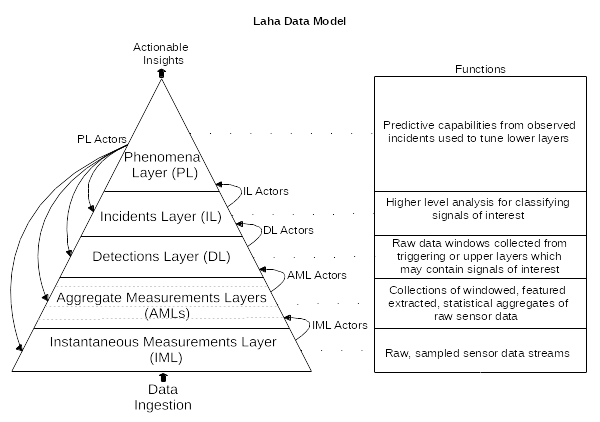
\includegraphics{figures/laha_abstract_overview.png}
	\label{laha-abstract-overview}
\end{figure}

The Laha framework aims to provide two important benefits to DSNs:
\begin{enumerate}
	\item Convert sensor data into actionable data and insights
	\item Provide graceful degradation and metrics on storage requirements for voluminous sensor data
\end{enumerate}

Although not the main focus of this dissertation, Laha provides several tangential benefits in the following DSN problem domains:

\begin{enumerate}
	\item Triggering optimizations
	\item Detection and classification optimizations
	\item Topological optimizations
	\item Sensor energy requirement optimizations
\end{enumerate}

These tangential benefits are provided by Laha Actors that exist within each level of the Laha framework. I don't claim that these techniques are novel, but I do claim that either all or a subset of these techniques are required to enable progress towards the main goals of this framework. To that end, Laha Actors implement several state of the art algorithms present in the literature that address these tertiary problems.

Laha is evaluated by designing and implementing two Laha-compliant reference implementations, OPQMauka and Lokahi. Open Power Quality (OPQ) is a power quality (PQ) network consisting of custom hardware and distributed software services that detect distributed PQ signals such as voltage sags and swells, frequency sags and swells, transients, THD, and other known PQ issues. OPQMauka is a distributed, plugin based middleware component of OPQ that performs higher level analysis, data management, and optimizations of the OPQ services. Lokahi is a distributed infrasound network consisting of mobile iOS and Android devices and multiple cloud based software services whose purpose is to supplement the International Monitoring System (IMS) in detecting large infrasound signals.

The reference implementations are designed and were deployed to test sites at UH Manoa and at the Infrasound Laboratory in Kailua-Kona, Big Island.

Data collected from the PQ network was validated against calibrated reference sensors that have already been installed at the power mains of a subset of buildings on campus. The Office of Energy Management at UH Manoa has given us full access to live and historic PQ data collected at these reference sensors. OPQBoxes were co-located and placed in buildings with the reference sensors so that I can validate that the triggering and raw data streams I receive from the OPQBoxes are in line with what the reference sensors are observing.

Data collected from the infrasound network was also validated against industry standard calibrated BNK infrasound sensors. Further, signals in the infrasound network are known a priori since I am able to control the signals that are generated from our calibrated infrasound source, allowing further validation of received signals.

In order to evaluate the generality of the Laha-framework, two separate Laha-compliant DSNs sensing different domains were designed, distributed, and evaluated. 

The first Laha-compliant DSN is Open Power Quality (OPQ), a distributed DSN that collects and analyzes power quality (PQ) signals. PQ is a measure of the ``goodness" of the power feeding your electronics. The features that this network collects includes voltage, frequency, and THD. From these features, OPQ can classify the following PQ signals: voltage dips/swells, frequency dips/swells, high levels of THD, and transients. Another goal of this network is to detect distributed PQ signals. That is, the same signal detected on multiple sensors to study how PQ signals move through a power grid. This network provides metrics on the number of incidents classified as well as numbers of correct predictions from Phenomena. The number of classified incidents are compared to industry standard PQ monitors co-located with OPQ sensors as a means of evaluating if Laha is capable of supporting the goals of this network.

The second Laha-compliant DSN is Lokahi, a distributed, mobile infrasound detection network. Infrasound consists of sounds waves that are less than 20 Hz. These signals are generated by large movements of the atmosphere and can be observed from large standoff distances. Examples of infrasound sources include volcano eruptions, meteors, missile launches, and large explosions. In this network, Android and iOS devices are deployed with a special app that is capable of collecting acoustic signals as they travel through the atmosphere. As part of the evaluation, in this network, we collected and discriminated infrasound signals from different types of infrasound sources. Many of these signals are correlated with industry standard infrasound sensors to show that Laha is capable of supporting the infrasound detection goals of this network.

In order to evaluate the multi-level representation of the Laha Framework in the context of providing actionable data, I setup experiments to produce cyclical and predictable signals and tested whether or not Laha is able to utilize predictive analytics to provide actionable insights. To test this, I provided the number of false positive and false negatives for predictive analytic results. I evaluated if the sensing domain has any effect on how well Laha is able to provide actionable insights. I also claim that each level in the Laha-hierarchy is important in the process of deriving these insights. I provide data that either supports or opposes the usefulness of each level, whether the current number of levels is adequate, and whether the idea of using level to provide actionable insight is useful at all.

I evaluated my claim that a tiered TTL approach to sensor data management provides the benefits of providing an configurable upper bounds on storage requirements for each Laha level, graceful degradation, and a reduction of sensor noise being stored. To test this, I implemented procedures for calculating storage bounds and determined if these theoretical bounds are valid in practice. Since it's possible that the TTL approach could throw away important data, I measured the number of false positives using the TTL approach as a means of evaluating its usefulness with a discussion of how detrimental these false positives might actually be to understanding and creating actionable data sets.

Finally, I evaluated multiple state of the art algorithms current in the literature for optimizing triggering, detection, classification, sensor energy usage, and topological modeling and provide metrics to their usefulness for making progress towards the larger goals of providing a generally useful representation for DSNs, converting primitive sensor data into actionable insights, and providing a tiered approach to DSN data management and storage requirements. I provide a discussion on whether these techniques are useful within the two domains that they are implemented, and if they are, how they contribute to the overall goals of this framework. We also show which combinations of tertiary techniques provide the most traction in solving the overall goals of this framework.

%To evaluate the five benefits from Laha, several different approaches are taken depending on the Laha deployment and the benefit being evaluated. In the UH Manoa PQ deployment, I will co-locate sensors in our deployment and for each metric, one of the sensors will use Laha's optimizations and the other sensor will not. This will provide metrics that allows us to compare and contrast our optimization techniques within the OPQ network. 
%
%In the Lokahi infrasound network, I will run a series of experiments where I can produce the same infrasound signals in each experiment and only change the tuning and optimizations that Laha applies to generate metrics for evaluation within the Laha network.
%
%When evaluating the five proposed benefits of Laha, I will specifically look at the following metrics. 
%
%For the tiered management of Big Data, I will measure the total amount of data saved and discarded at each level of the Laha data hierarchy while providing an upper bound of required storage for the given state of the network. I will also look at how the number of false positives and false negatives change when using Laha's tiered data management versus a ``store everything" approach. 
%
%When evaluating automatically provided context of classified incident I will measure the number of Incidents that are correctly identified or not identified as a metric of false positives and false negatives respectively.
%
%In order to evaluate optimization of triggering, I will measure false positives and false negatives of triggered events. I will also evaluate if optimized triggering provides any benefits to overall bandwidth usage and sensor power requirements of the DSN.
%
%To evaluate optimization of detection and classification of Incidents I will measure the signal-to-noise ration of detection windows to determine if optimizing of detections increases the signal-to-noise ration. To evaluate classifications of Incidents, I will record the number of false positives and false negative when the network is optimized versus when the network in unoptimized.
%
%Finally, to evaluate sensor field topology, Laha will output a statistical model of signals distances between every pair of sensors in the DSN. These distances will be compared to the ground truth signal distances provided before hand. If  Laha is able determine the sensing field topology, I will evaluate if the model can be used to further refine and optimize lower levels of the Laha hierarchy.

I expect to deploy reference implementations before the end of 2018 with validated data collection beginning and continuing through Q3 2019. I anticipate writing my dissertation along side the deployment and data collection process and to be finished in Q3 2019.

\section{Anticipated contributions of Laha}
Laha hopes to make the following four contributions to the areas of DSNs and specially optimization and management of DSNs.  First, the Laha design, a novel abstract distributed sensor network that provides two useful properties relating to data management, converting primitive data to actionable data and tiered management of Big Data.

Second, an evaluation of the Laha abstract framework through the deployment of two Laha-compliant reference implementations, validated data collection, and several experiments that are used to either confirm or deny the benefits touted by Laha. 

Third, two Laha-compliant reference implementations, OPQ and Lokahi, which can be used to form DSNs for the collection of distributed power quality signals and the distributed collection of infrasound signals.

Fourth, an evaluation of state of the art algorithms in practice and a discussion of their usefulness as applied to two different DSN domains.

Fifth, a set of implications for modern distributed sensor networks as a result of the evaluation of Laha. That is, how does the confirmation of denial of Laha's benefits affect the field of modern DSNs moving forward?





